\section{Numerische Auswertung}
\label{sec:verfahrensvergleich}
Wir werden nun die numerischen Verfahren zur Lösung von Anfangswertproblemen mit dem Verfahren des maschinellen Lernens
miteinander vergleichen. Es werden hierfür die Python Bibliotheken \textit{numpy}\footnote{URL: \url{https://numpy.org/}},
\textit{scipy} \footnote{URL: \url{https://scipy.org/}} für numerische Verfahren und \textit{tensorflow}
\footnote{URL: \url{https://www.tensorflow.org/}} für die Architektur der neuronalen Netze verwendet. Das gegebene
Anfangswertproblem wird zuerst mithilfe des \textit{4-5-Runge-Kutta-Verfahrens} beziehungsweise des BDF-Verfahrens
gelöst und danach mit einem neuronalen Netz approximiert. Die folgenden Ergebnisse werden darauffolgend anhand
verschiedenen Maßen verglichen. Dabei werden unter anderem die \textit{Trajektorien} der berechneten Lösungen betrachtet.
Eine Trajektorie ist hierbei das Bild $T(x_0):= \{x(t,x_0): t\in I_{\text{max}}\}$ der Lösung des Anfangswertproblems
\eqref{first-order-num}, wobei $I_{\text{max}}$ das maximale Existenzintervall ist. Des Weiteren werden wir den globalen
Fehler des numerischen Verfahrens $\left\lVert x(t_i) - u_i \right\rVert_2$ mit dem globalen Fehler der neuronalen Netze
$\left\lVert x(t_i) - \hat{x}(t_i) \right\rVert_2$ in Abhängigkeit der Zeit $t_i=t_0 + ih$ und vergleichen. Dabei
ist zu beachten, dass eine exakte Lösung $x$ vorliegen muss. In dem Abschnitt \ref{subsec:rebound-Pendel} ist das
analytische Berechnen der Lösung aufwendig, weshalb es nicht möglich ist, die globalen Fehler zu vergleichen. Deshalb
werden wir ein Runge-Kutta-Verfahren mit sehr kleiner Schrittweite verwenden, um eine Referenzlösung zu berechnen.
Hierbei betrachten wir sowohl die Trajektorien, als auch den Graph der ersten Komponente
der berechneten Lösung in Abhängigkeit der Zeit.
Zuletzt geben wir die Kostenfunktion der neuronalen Netze in Abhängigkeit der Epochen und, wenn möglich, den globalen
Fehler für das gesamte Zeitintervall in Abhängigkeit der Epochen an. Dabei wenden wir den sogenannten
\textit{gleitenden Mittelwert} an, um die Oszillation der beiden Graphen durch die Varianzen der Batches, zu
minimieren. Hierbei sind sprunghafte Änderungen der Kostenfunktion und des Fehlers gemeint, die entstehen, sobald neue
Zufallszahlen gewählt werden und das Netzwerk noch nicht angepasst wurde. Hierzu verwenden wir die Funktion
\textit{pandas.DataFrame.mean} der Bibliothek \textit{pandas}, für die Dokumentation siehe \cite{PandasDataFrameMean}.
Für das 4-5-Runge-Kutta-Verfahren verwenden wir die Bibliothek \texttt{scipy.integrate}, genauer die Funktion
\texttt{scipy.integrate.RK45},  siehe \cite{ScipyIntegrateRK45}. Die Berechnungen wurden mit einem AMD Ryzen 7 5800X CPU,
32GB RAM und einer NVIDIA RTX 3060 Ti GPU durchgeführt. Der Quellcode zur Lösung der folgenden Anfangswertproblemen mit
numerischen Verfahren und die Implementierung der neuronalen Netze befindet sich auf dem beigelegtem Datenträger.
\newpage

\subsection{Rebound-Pendel}
\label{subsec:rebound-Pendel}
Das Rebound-Pendel \cite[6-7]{flamantSolvingDifferentialEquations2020} ist ein System, in dem ein Pendel an einer
Seite auf eine gedämpfte Feder treffen kann, siehe \ref{fig:rebound_pendulum_diagram}.
\begin{figure}
       \centering
       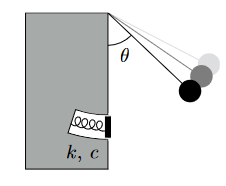
\includegraphics{rebound_pendulum_diagram}
       \caption{Diagramm eines Rebound Pendels\cite[6]{flamantSolvingDifferentialEquations2020}}
       \label{fig:rebound_pendulum_diagram}
\end{figure}
Das zugehörige Anfangsproblem zweiter Ordnung hat die Form
\begin{align*}
       \theta^{\prime \prime} &= - \frac{g}{l} \sin(\theta) + H(-\theta)
       \text{ReLU}(-\frac{kl}{m}\theta - c \theta^{\prime})\\
       \theta(0) &= 1, \quad \theta^{\prime}(0)=0.2
\end{align*}
mit dem Auslenkungswinkel $\theta$. Mit der Einführung der Winkelgeschwindigkeit $\varphi=\theta^{\prime}$ kann dieses
Problem zu einem System erster Ordnung
\begin{align}
       \theta^{\prime} &= \varphi, \nonumber \\
       \varphi^{\prime} &= - \frac{g}{l} \sin(\theta) + H(-\theta)
       \text{ReLU}(-\frac{kl}{m}\theta - c \varphi), \label{rebound-pendulum}\\
       \theta(0) &= 1, \quad \varphi(0)=0.2 \nonumber
\end{align}
umgeschrieben werden. Hierbei ist $\text{ReLU}(x)= \max(x, 0)$,
\begin{align*}
       H(x) =
       \begin{cases}
              0, &x<0 \\
              1, &x \geq 0
       \end{cases}
\end{align*}
die \textit{Heavside}-Funktion,
$g$ die Erdbeschleunigung, $l$ die Länge des Pendels, $m$ die Masse des Pendels, $k$ die Federkonstante und $c$ der
Dämpfungskoeffizient. Wir werden dieses System nun in dem Zeitraum $t \in [0, 10]$ lösen bzw. approximieren und die
Resultate vergleichen. Für beide Verfahren werden zur Vereinfachung $g=1$ und $l=1$ gesetzt. Außerdem wird für das
Runge-Kutta-Verfahren $k=3$ und $c=1$ gewählt. Für die Funktionen zur Berechnung der Lösungen mithilfe der
Runge-Kutta-Verfahren werden die relative Toleranz $rtol=10^{-5}$ und die absolute Toleranz $atol=10^{-7}$ gesetzt.
Die Referenzlösung wird mit Hilfe $scipy.integrate.RK45$-Funktion mit $rtol=atol=10^{-14}$ berechnet.
\begin{table}
       \renewcommand{\arraystretch}{1.0}
       \centering
       \begin{tabular}{ l | l }
              \hline
              Netzwerkstruktur & \\
              \hline
              Anzahl der Schichten & $L=10$ \\
              Eingabeschicht & $n^{(0)}=5$ mit $\Phi(x)=\tanh(x)$ \\
              Versteckte Schichten & $n^{(l)}=128$, $l = 1, \dots, L-1$ mit $\Phi(x)=\tanh(x)$ \\
              Ausgabeschicht & $n^{(L)}=2$ mit $\Phi(x)=x$ \\
              \hline
              Hyperparameter und Initialisierungsintervalle & \\
              \hline
              Anfangswertbereiche & $(\theta_0, \varphi_0) \in [0.0, 1.0] \times [-0.2, 0.2]$ \\
              Paramaterbereiche & $(k, c) \in [2.0, 5.0] \times [0.0, 2.0]$ \\
              Zeitraum & $t \in [0, 10]$ \\
              \hline
              Optimierung & \\
              \hline
              Gradientenverfahren & Adam \\
              Gewichtsfunktion & $b(t)=e^{-0.5t}$ \\
              Batch Size & $|B|=10000$ \\
              Epochen & $100000$ \\
              Lernrate & $\eta= 0.0001$ \\
              Gewichtsinitialisierung & Xavier-Initialisierung \\
              \hline
              Statistiken & \\
              \hline
              Trainingrate & 9 Batches/Sekunde  \\
              Trainingszeit & 3.1 Stunden \\
              \hline
       \end{tabular}
       \caption{Netzwerkstruktur, Hyperparameter, Initialisierungsintervalle, Optimierungsparameter und Statistiken
       für das Rebound-Pendel-Anfangswertproblem.}
\label{rebound-pendulum-table}
\end{table}
In Tabelle \ref{rebound-pendulum-table} sind alle relevanten Daten für das Rebound-Pendel-Anfangswertproblem gegeben,
wobei $\Phi$ die Aktivierungsfunktion für die jeweiligen Schichten des neuronalen Netzes ist. Wie bereits erwähnt, haben
wir keine exakte Lösung vorliegen, weshalb wir die berechneten Lösungen mit der Referenzlösung vergleichen.
In Abbildung \ref{fig:rebound-trajectories} sehen wir, dass sich die beiden Trajektorien einen ähnlichen
Verlauf haben. Jedoch sind die Trajektorien des Runge-Kutta-Verfahrens viel näher an der Vergleichstrajektorie.
Ähnliches lässt sich in Abbildung \ref{fig:rebound-trajectories-in-time} beobachten, dass sowohl die Trajektorie des
des maschinellen Lernens als auch die Trajektorie des Runge-Kutta-Verfahrens einen ähnlichen Verlauf wie die
Referenzlösung haben. Es fällt aber auf, dass das Runge-Kutta-Verfahren näher an der Trajektorie der Referenzlösung ist,
als die Approximation des neuronalen Netzes. In Abbildung \ref{fig:rebound-loss} befindet sich die Entwicklung der
Kostenfunktion bei steigenden Epochen. Man kann beobachten, dass die Werte der Kostenfunktion bei hohen Epochen wieder
steigt. Dies zeigt, dass eine Erhöhung der Epochen ohne Anpassung anderer Hyperparameter, wie beispielsweise der
Lernrate, nicht zielführend für eine Verbesserung der Approximation sein kann. Zuletzt zeigt die Rechenzeit des
Runge-Kutta-Verfahrens von $0.22$ Sekunden, sowie die Rechenzeit der Referenzlösung von $0.18$ Sekunden, dass im
Vergleich zu der Trainingszeit des neuronalen Netzes von $3.1$ Stunden um ein Vielfaches kleiner ist. Zusammenfassend
erkennen wir, dass das Runge-Kutta-Verfahren im Vergleich zu dem neuronalen Netz ein besseres Ergebnis mit viel
kleineren Rechenzeiten liefert und sobald wir die relative und absolute Toleranz verringern, kann dieses Ergebnis
optimiert werden.
\begin{figure}
       \centering
       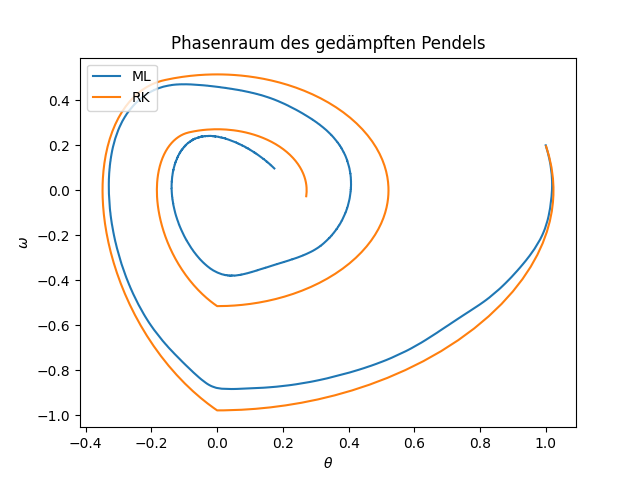
\includegraphics[scale=0.8]{Rebound_plots/reboundpendulumtrajectories_}
       \caption{Trajektorie der verschiedenen Lösungen.}
       \label{fig:rebound-trajectories}
\end{figure}
\begin{figure}
       \centering
       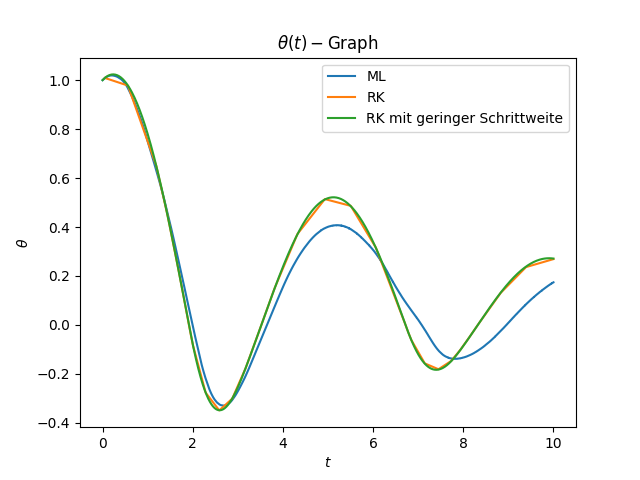
\includegraphics[scale=0.8]{Rebound_plots/reboundpendulumtrajectories_in_time_}
       \caption{$(t, \theta(t))$ Graph der berechneten Lösungen.}
       \label{fig:rebound-trajectories-in-time}
\end{figure}
\begin{figure}
       \centering
       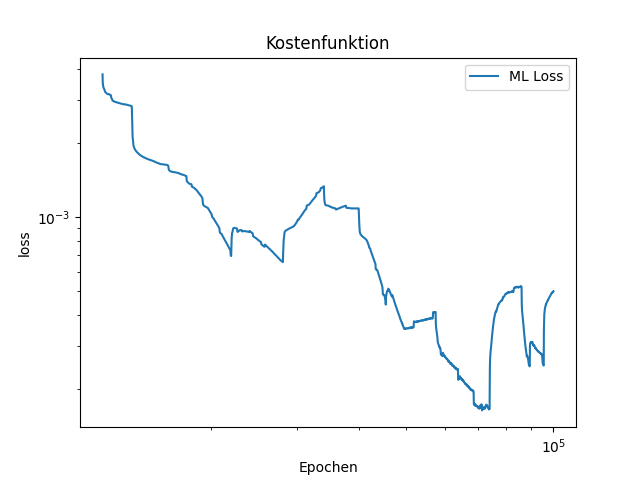
\includegraphics[scale=0.8]{Rebound_plots/reboundpendulumavr_loss}
       \caption{Kostenfunktion des neuronalen Netzes bei steigender Epochenanzahl.}
       \label{fig:rebound-loss}
\end{figure}
\clearpage

\subsection{Steife Differentialgleichung}
\label{sec:steife-differentialgleichung}
Das Anfangswertproblem (siehe \cite[173]{stoerNumerischeMathematik2005})
\begin{align}
       \label{stiff}
       x_{1}^{\prime} &= \frac{1}{2} ((\lambda_1 + \lambda_2)x_1 + (\lambda_1 - \lambda_2)x_2), \nonumber \\
       x_{2}^{\prime} &= \frac{1}{2} ((\lambda_1 - \lambda_2)x_1 + (\lambda_1 + \lambda_2)x_2), \\
       x_1(0) &= c_1 + c_2, \quad x_2(0) = c_1 - c_2 \nonumber
\end{align}
lässt sich mit der Matrix
\[
       A = \frac{1}{2}
       \begin{bmatrix}
                \lambda_1 + \lambda_2 & \lambda_1 - \lambda_2 \\
                \lambda_1 - \lambda_2 & \lambda_1 + \lambda_2
       \end{bmatrix}
\]
zu
\begin{align*}
       x^{\prime} &= Ax, \\
       x(0) &=
       \begin{bmatrix}
              c_1 + c_2 \\
              c_1 - c_2
       \end{bmatrix}
\end{align*}
umformulieren. Dabei betrachten wir $\lambda_1, \lambda_2 < 0$ und $c_1, c_2 \in \mathbb{R}$. Die Matrix A hat die
Eigenwerte $\lambda_1$ und $\lambda_2$ und für $\lambda_1 = -100$ und $\lambda_2 = -1$ ist
das Anfangswertproblem \ref{stiff} nach Definition \eqref{steife-dgl} $steif$. Da \eqref{stiff} eine lineare
Differentialgleichung erster Ordnung ist, können wir die Lösung mithilfe \eqref{linear-ode-solution} angeben:
\[
       x(t) =
       \begin{bmatrix}
              c_1 e^{\lambda_1 t} + c_2 e^{\lambda_2 t} \\
              c_1 e^{\lambda_1 t} - c_2 e^{\lambda_2 t}
       \end{bmatrix}.
\]
Der erste Eigenwert $\lambda_1$ lässt den ersten Summand der Lösung viel schneller gegen $0$ konvergieren für
$t \rightarrow \infty$, als der zweite Eigenwert $\lambda_2$. Wir verwenden nun das explizite Euler-Verfahren der Form
\begin{align*}
       u_0 &= x_0 \\
       u_i &= u_{i-1} + hAu_{i-1}= \dots = (I + hA)^{i}u_0, \qquad i=1,\dots,N
\end{align*}
um das Anfangswertproblem zu lösen. Die numerische Lösung ist also gegeben durch
\begin{align*}
       u_{i}=
       \begin{bmatrix}
              c_1 (1+h\lambda_1)^{i} + c_2 (1+h\lambda_2)^{i}\\
              c_1 (1+h\lambda_1)^{i} + c_2 (1+h\lambda_2)^{i}
       \end{bmatrix}.
\end{align*}
Damit die exakte Lösung und die numerische Lösung das gleiche Grenzverhalten besitzen, muss $|1 + h\lambda_1|<1$ und
$|1 + h\lambda_2|<1$ gelten. Hieraus resultieren Bedingungen für $h$, also eine Schrittweitenbeschränkung der Form
$h<\frac{2}{|\lambda_1|}$ und $h<\frac{2}{|\lambda_2|}$. Da $|\lambda_2| \ll |\lambda_1|$, bestimmt der erste Eigenwert
über die Beschränkung der Schrittweite, obwohl dieser in der exakten Lösung für größere Zeiten $t$ fast keinen Einfluss
hat. Wir werden sehen, dass dieses Problem auch im Runge-Kutta-Verfahren auftreten wird, weshalb wir außerdem ein
\textit{BDF-Verfahren}, also ein Mehrschrittverfahren, verwenden werden, um die Ergebnisse mit dem Verfahren der
Lösungspakete vergleichen zu können. Für alle Verfahren setzen wir $c_1=3$, $c_2=4$, $\lambda_1 = -100$ und $\lambda_2=-1$.
Für die Implementierung des BDF-Verfahrens wird die Funktion \texttt{scipy.integrate.BDF}, siehe
\cite{ScipyIntegrateBDF}, verwendet. Für beide Verfahren setzen wir dazu die relative Toleranz $rtol=10^{-2}$ und die
absolute Toleranz $atol=10^{-7}$, um die steife Eigenschaft des gegebenen Anfangswertproblems \eqref{stiff} beobachten
zu können. Ähnlich wie in Abschnitt \ref{subsec:rebound-Pendel} sind in Tabelle \ref{stiff-table} alle relevanten Daten
zu dem verwendeten neuronalen Netz für \eqref{stiff} gegeben.
\begin{table}
       \renewcommand{\arraystretch}{1.0}
       \centering
       \begin{tabular}{ l | l }
              \hline
              Netzwerkstruktur & \\
              \hline
              Anzahl der Schichten & $L=10$ \\
              Eingabeschicht & $n^{(0)}=5$ mit $\Phi(x)=\tanh(x)$ \\
              Versteckte Schichten & $n^{(l)}=32$, $l = 1, \dots, L-1$ mit $\Phi(x)=\tanh(x)$ \\
              Ausgabeschicht & $n^{(L)}=2$ mit $\Phi(x)=x$ \\
              \hline
              Hyperparameter und Initialisierungsintervalle & \\
              \hline
              Anfangswertbereiche &
              $x_{1,0} \in [c_1+c_2 - 0.05, c_1+c_2 + 0.05]$ \\
              & $x_{2,0} \in [c_1-c_2 - 0.05, c_1-c_2 + 0.05]$ \\
              Paramaterbereiche &
              $\lambda_1 \in [\lambda_1 - 0.05, \lambda_1 + 0.05]$ \\
              & $\lambda_2 \in[\lambda_2 - 0.05, \lambda_2 + 0.05]$ \\
              Zeitraum & $t \in [0, 10]$ \\
              \hline
              Optimierung & \\
              \hline
              Gradientenverfahren & Adam \\
%              Gewichtsfunktion & $b(t)=e^{-0.5t}$ \\
              Gewichtsfunktion & $b(t)=1$ \\
              Batch Size & $|B|=10000$ \\
              Epochen & $1000000$ \\
              Lernrate & $\eta= 0.0001$ \\
              Gewichtsinitialisierung & Xavier-Initialisierung \\
              \hline
              Statistiken & \\
              \hline
              Trainingrate & 125 Batches/Sekunde \\
              Trainingszeit & 2.22 Stunden \\
              \hline
       \end{tabular}
       \caption{Netzwerkstruktur, Hyperparameter, Initialisierungsintervalle, Optimierungsparameter und Statistiken
       für das steife Anfangswertproblem \eqref{stiff}.}
       \label{stiff-table}
\end{table}
In Abbildung \ref{fig:stiff-trajectories} können wir den Verlauf der Trajektorie mit dem Anfangspunkt
$x(0)=(7,-1)^{\intercal}$ für die erwähnten Verfahren betrachten. Wie bereits besprochen beschränkt der betragsmäßig große
Eigenwert $\lambda_1=-100$ die Schrittweite $h$, was zu einer ungenauen Lösung des Runge-Kutta-Verfahren führt. Die
Approximation des neuronalen Netzes jedoch lässt sich mit der Lösung des BDF-Verfahrens vergleichen, da es für ein
gewissen Zeitintervall sogar einen niedrigeren globalen Fehler hat als die Lösung des BDF-Verfahrens, siehe
\ref{fig:stiff-error-in-time}. Es fällt auf, dass während in Abbildung \ref{fig:stiff-trajectories} der Fehler für das
Runge-Kutta-Verfahren viel größer als der Fehler des BDF-Verfahrens scheint, so ist der Fehler der beiden Verfahren in
Abbildung \ref{fig:stiff-error-in-time} vergleichbar. Das liegt daran, dass die Abbildung der Trajektorien fehlleitend
ist, da wir nicht erkennen können, zu welchem Zeitpunkt die Koordinaten der Trajektorien gehören. Mit der exakten Lösung
\[
       x(t) = \begin{bmatrix*} 3 e^{-100 t} + 4 e^{- t} \\
              3 e^{-100 t} - 4 e^{-t} \end{bmatrix*}
\]
können wir sehen, dass die Trajektorien beispielsweise bei einem Zeitpunkt $t=5 \in [0, 10]$ die Koordinaten
$(0.027, -0.027)$ hat. Also befinden wir nach dem halben Zeitintervall in der Nähe vom Ursprung $(0,0)$. Deshalb müssen
wir in Abbildung \ref{fig:stiff-error-in-time} den Fehler in Abhängigkeit der Zeit für $t<5$ betrachten, um die
Verhalten der Trajektorien in Abbildung \ref{fig:stiff-trajectories} wiederzufinden. Dabei sehen wir in beiden
Abbildungen, dass das neuronale Netz das beste Ergebnis liefert.
Der oszillierende Fehler des Runge-Kutta-Verfahrens stimmt mit dem Verhalten der Trajektorie überein. Des Weiteren fällt
auf, dass der Fehler des neuronalen Netzes über die Zeit nahezu konstant bleibt, während der Fehler der anderen
Verfahren im Laufe der Zeit sinkt. Zudem sehen wir in Abbildungen \ref{fig:stiff-error} und \ref{fig:stiff-loss} den
Verlauf des globalen Fehlers und der Kostenfunktion für steigende Epochen. Hierbei bemerken wir, dass für das Minimum
der Kostenfunktion in Abbildung \ref{fig:stiff-loss} die Größenordnung $10^2$ hat, was im Vergleich zu der
Kostenfunktion in Abschnitt \ref{subsec:rebound-Pendel} (siehe Abbildung \ref{fig:rebound-loss}) um $5$ Größenordnungen
übersteig. Das hat den Grund, dass der betragsmäßig große Eigenwert $\lambda_1=-100$ für erhöhte Werte der Kostenfunktion
sorgt, da diese von der gegebenen Differentialgleichung \eqref{stiff} abhängt.
Sowohl der globale Fehler als auch die Kostenfunktion sinken wie erwartet bei steigender Epochenzahl, jedoch wird die
Steigung beider Graphen betragsmäßig kleiner. Um eine genauere Approximation zu erhalten, müssten wir die Anzahl der
Epochen erhöhen, wobei dies zu einer Laufzeit von $2.2$ Stunden übersteigt. Das BDF-Verfahren hat trotz einer
Beschränkung der absoluten und relativen Toleranz das Anfangswertproblem in $0.039$ Sekunden mit akzeptablen
Fehler approximiert. Deshalb können wir zusammenfassend sagen, dass das BDF-Verfahren allgemein besser zur Lösung
von steifen Anfangswertproblemen geeignet ist.
\begin{figure}
       \centering
       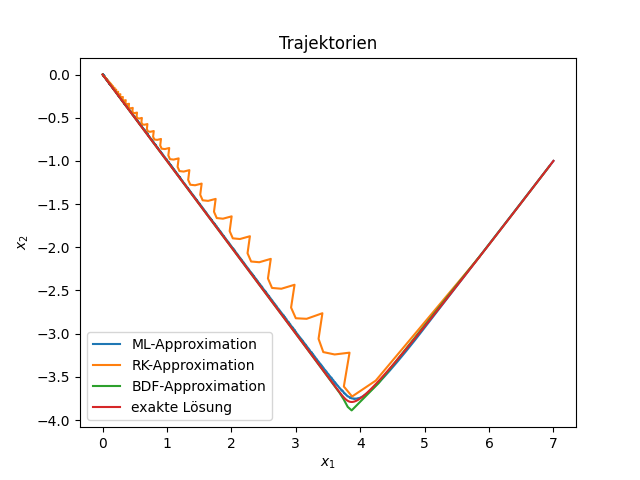
\includegraphics[scale=0.8]{Stiff_plots/stifftrajectories_}
       \caption{Trajektorien der verschiedenen Lösungen.}
       \label{fig:stiff-trajectories}
\end{figure}
\begin{figure}
       \centering
       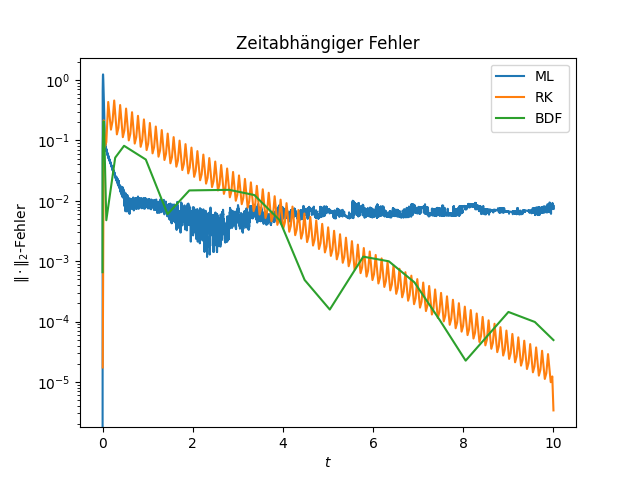
\includegraphics[scale=0.8]{Stiff_plots/stiffError_in_time}
       \caption{Globaler Fehler  der jeweiligen Verfahren in Abhängigkeit der Zeit.}
       \label{fig:stiff-error-in-time}
\end{figure}
\begin{figure}
       \centering
       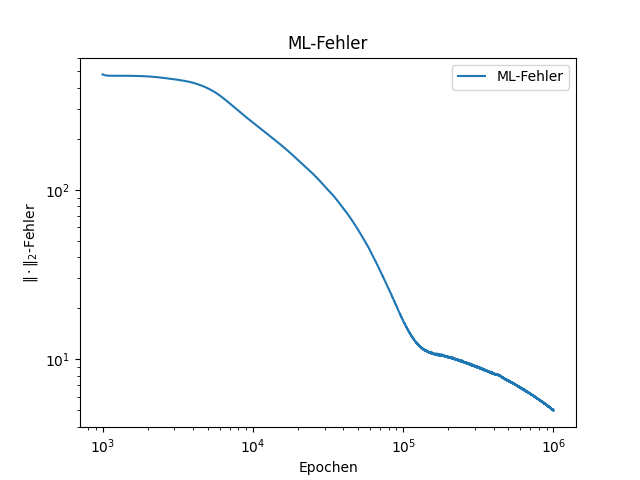
\includegraphics[scale=0.8]{Stiff_plots/stiffML_error_}
       \caption{Globaler Fehler für steigende Epochen.}
       \label{fig:stiff-error}
\end{figure}
\begin{figure}
       \centering
       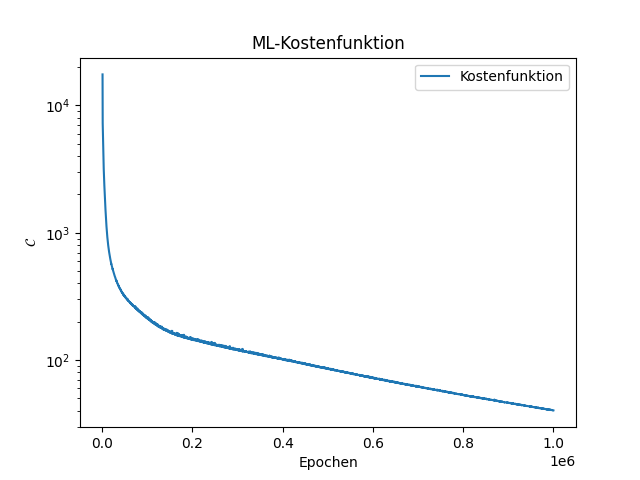
\includegraphics[scale=0.8]{Stiff_plots/stiffML_Loss_}
       \caption{Kostenfunktion für steigende Epochen.}
       \label{fig:stiff-loss}
\end{figure}
\clearpage

\subsection{Harmonischer Oszillator}
\label{sec:harmonischer-oszillator}
Zuletzt werden wir die Lösung für den harmonischen Oszillator \cite[8]{flamantSolvingDifferentialEquations2020} mit
verschiedenen Netzwerkstrukturen approximieren und die Ergebnisse untereinander und mit dem 4-5-Runge-Kutta-Verfahren
vergleichen. Die Bewegung eines harmonischen Oszillators ist gegeben durch
\begin{align}
       \label{harmonic-oscillator}
       &x^{\prime}=v, \qquad v^{\prime}=-\frac{k}{m}x, \\
       &x(0)=0, \quad v(0)=0, \nonumber
\end{align}
wobei zur Vereinfachung $m=1$ gesetzt wird. Außerdem gilt für das Runge-Kutta-Verfahren $k=1$, für relative Toleranz
$rtol = 10^{-10}$ und die absolute Toleranz $atol = 10^{-14}$. Die Tabelle \ref{stiff-table-data} enthält alle Daten
für die folgenden neuronale Netze verwendet werden.
\begin{table}
       \renewcommand{\arraystretch}{1.0}
       \centering
       \begin{tabular}{ l | l }
              \hline
              Hyperparameter und Initialisierungsintervalle & \\
              \hline
              Anfangswertbereiche &
              $(x_{0},v_0) \in [-1.0, 1.0] \times [-1.0, 1.0]$ \\
              Paramaterbereiche & $k \in [0.5, 2.0]$ \\
              Zeitraum & $t \in [0, 2\pi]$ \\
              \hline
              Optimierung & \\
              \hline
              Gradientenverfahren & Adam \\
              Gewichtsfunktion & $b(t)=1$ \\
              Batch Size & $|B|=10000$ \\
              Epochen & $100000$ \\
              Lernrate & $0.0001$ \\
              Gewichtsinitialisierung & Xavier-Initialisierung \\
              \hline
       \end{tabular}
       \caption{Hyperparameter, Initialisierungsintervalle und Optimierungsparameter für den harmonischen Oszillator
       \eqref{harmonic-oscillator}.}
       \label{stiff-table-data}
\end{table}
\clearpage
Wir werden zuerst eine konstante Anzahl der Schichten $L=6$ verwenden und die Anzahl der Neuronen pro Schicht variieren.
Dazu betrachten wir versteckte Schichten mit den Längen
$n^{(l)} = 4,$ $8,$ $16,$ $32$, für $l = 1, \dots, L-1$. Tabelle \ref{stiff-table-first} enthält die genauen
Netzwerkstrukturen.
\begin{table}
       \renewcommand{\arraystretch}{1.0}
       \centering
       \begin{tabular}{ l | l }
              \hline
              Netzwerk 1 & \\
              \hline
              Anzahl der Schichten & $L=6$ \\
              Eingabeschicht & $n^{(0)}=4$ mit $\Phi(x)=\tanh(x)$ \\
              Versteckte Schichten & $n^{(l)}=4$, $l = 1, \dots, L-1$ mit $\Phi(x)=\tanh(x)$ \\
              Ausgabeschicht & $n^{(L)}=2$ mit $\Phi(x)=x$ \\
              Lernrate & $\eta=0.0001$ \\
              Trainingrate & 195 Batches/Sekunde \\
              Traningszeit & 0.14 Stunden \\
              \hline
              Netzwerk 2 & \\
              \hline
              Anzahl der Schichten & $L=6$ \\
              Eingabeschicht & $n^{(0)}=4$ mit $\Phi(x)=\tanh(x)$ \\
              Versteckte Schichten & $n^{(l)}=8$, $l = 1, \dots, L-1$ mit $\Phi(x)=\tanh(x)$ \\
              Ausgabeschicht & $n^{(L)}=2$ mit $\Phi(x)=x$ \\
              Lernrate & $\eta=0.0001$ \\
              Trainingrate & 195 Batches/Sekunde \\
              Trainingszeit & 0.14 Stunden \\
              \hline
              Netzwerk 3 & \\
              \hline
              Anzahl der Schichten & $L=6$ \\
              Eingabeschicht & $n^{(0)}=4$ mit $\Phi(x)=\tanh(x)$ \\
              Versteckte Schichten & $n^{(l)}=16$, $l = 1, \dots, L-1$ mit $\Phi(x)=\tanh(x)$ \\
              Ausgabeschicht & $n^{(L)}=2$ mit $\Phi(x)=x$ \\
              Lernrate & $\eta=0.0001$ \\
              Trainingrate & 195 Batches/Sekunde \\
              Trainingszeit & 0.14 Stunden \\
              \hline
              Netzwerk 4 & \\
              \hline
              Anzahl der Schichten & $L=6$ \\
              Eingabeschicht & $n^{(0)}=4$ mit $\Phi(x)=\tanh(x)$ \\
              Versteckte Schichten & $n^{(l)}=32$, $l = 1, \dots, L-1$ mit $\Phi(x)=\tanh(x)$ \\
              Ausgabeschicht & $n^{(L)}=2$ mit $\Phi(x)=x$ \\
              Lernrate & $\eta=0.0001$ \\
              Trainingrate & 180 Batches/Sekunde \\
              Trainingszeit & 0.15 Stunden \\
              \hline
       \end{tabular}
       \caption{Netzwerkstrukuren der ersten Variation.}
       \label{stiff-table-first}
\end{table}
In Abbildung \ref{fig:harmonic-neurons-variable-loss} und Abbildung \ref{fig:harmonic-neurons-variable-error} lässt
sich leicht erkennen, dass das bei steigender Anzahl der Neuronen sowohl die Kostenfunktion als auch der globale Fehler
das größte Minimum erreicht. Auch in Abbildung \ref{fig:harmonic-neurons-variable-trajectories} mit den Trajektorien
und in Abbildung \ref{fig:harmonic-neurons-variable-trajectories-in-time} mit den $x(t)$-Graphen
sehen wir, dass das neuronale Netz mit den meisten Neuronen pro Schicht die beste Lösung liefert. Die Lösung des
Runge-Kutta-Verfahrens approximiert die exakte Lösung jedoch viel besser, da die Trajektorie direkt unter der
Trajektorie der exakten Lösung liegt. Dies sieht man auch in Abbildung \ref{fig:harmonic-neurons-variable-error} mit den
globalen Fehler der Netzwerke, denn diese erreichen die minimale Größenordnung $10^0$. In Abbildung
\ref{fig:harmonic-neurons-variable-error-in-time} ist zu erkennen, dass der globale Fehler für die einzelnen
Zeitpunkte für das Runge-Kutta-Verfahren um $4$ Größenordnungen kleiner ist.
\begin{figure}
       \centering
       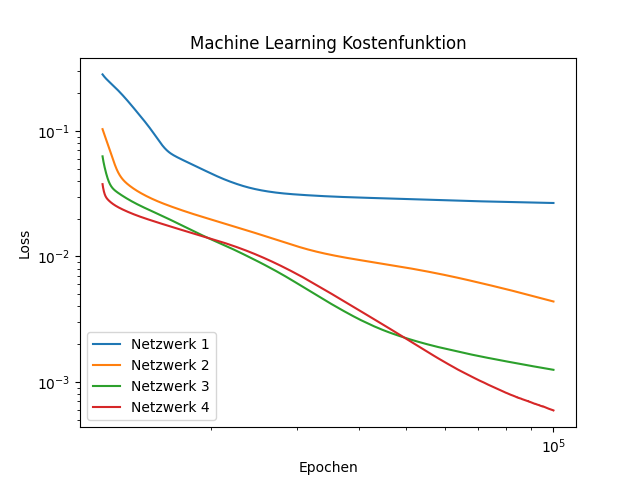
\includegraphics[scale=0.8]{harmonicoscillator_plots/harmonicoscillatorML_error__neurons_var_avrloss}
       \caption{Kostenfunktion der verschiedenen neuronalen Netze.}
       \label{fig:harmonic-neurons-variable-loss}
\end{figure}
\begin{figure}
       \centering
       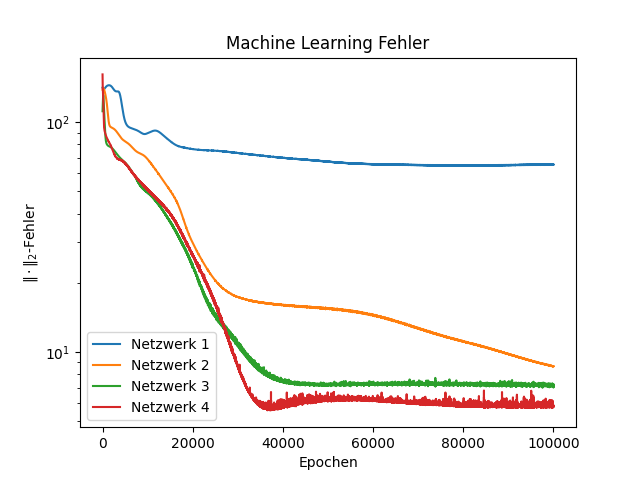
\includegraphics[scale=0.8]{harmonicoscillator_plots/harmonicoscillatorML_error__neurons_var_error}
       \caption{Globaler Fehler der verschiedenen neuronalen Netze.}
       \label{fig:harmonic-neurons-variable-error}
\end{figure}
\begin{figure}
       \centering
       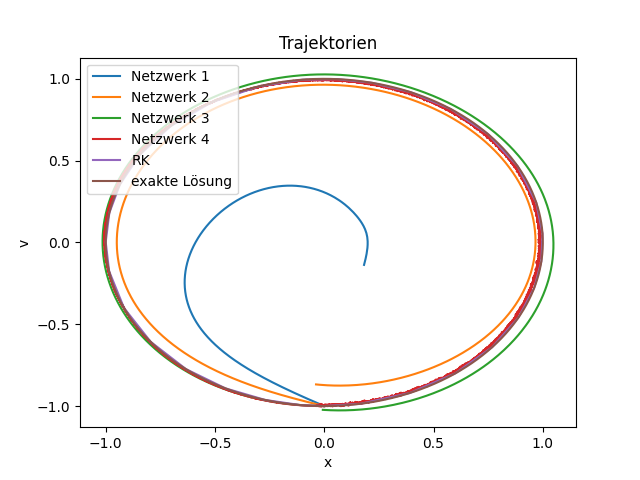
\includegraphics[scale=0.8]{harmonicoscillator_plots/harmonicoscillator_neurons_vartrajectories}
       \caption{Trajektorien der von den verschiedenen neuronalen Netzen approximierte Lösung, der Runge-Kutta-Lösung
       und der exakten Lösung.}
       \label{fig:harmonic-neurons-variable-trajectories}
\end{figure}
\begin{figure}
       \centering
       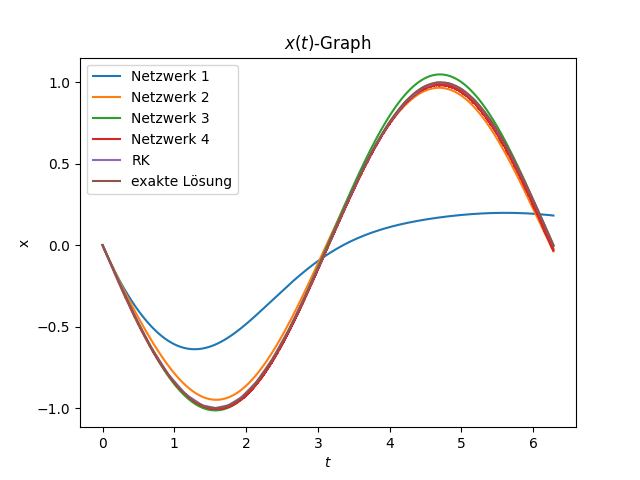
\includegraphics[scale=0.8]{harmonicoscillator_plots/harmonicoscillator_neurons_vartrajectories_in_time_}
       \caption{$(t,x(t))$ Graph der Lösungen des Runge-Kutta-Verfahrens, der Approximation der
       Lösungspakete und der exakten Lösung.}
       \label{fig:harmonic-neurons-variable-trajectories-in-time}
\end{figure}
\begin{figure}
       \centering
       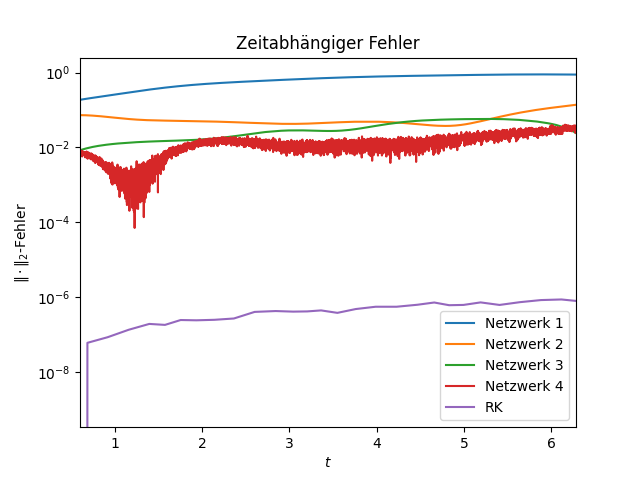
\includegraphics[scale=0.8]{harmonicoscillator_plots/harmonicoscillatorError_in_time_neurons_var}
       \caption{Globaler Fehler von Netzwerken $1$ bis $4$ und dem Runge-Kutta-Verfahren in Abhängigkeit der Zeit.}
       \label{fig:harmonic-neurons-variable-error-in-time}
\end{figure}
\clearpage
Nun werden wir die Netzwerke mit $4$, $8$ und $16$ versteckten Schichten vergleichen. Dazu wird die Länge der jeweiligen
Schichten $n^{(l)}=32$. Genauere Angaben zu den Netzwerken befinden sich in Tabelle \ref{stiff-table-second}.
\begin{table}
       \renewcommand{\arraystretch}{1.0}
       \centering
       \begin{tabular}{ l | l }
              \hline
              Netzwerk 1 & \\
              \hline
              Anzahl der Schichten & $L=6$ \\
              Eingabeschicht & $n^{(0)}=4$ mit $\Phi(x)=\tanh(x)$ \\
              Versteckte Schichten & $n^{(l)}=32$, $l = 1, \dots, L-1$ mit $\Phi(x)=\tanh(x)$ \\
              Ausgabeschicht & $n^{(L)}=2$ mit $\Phi(x)=x$ \\
              Lernrate & $\eta=0.0001$ \\
              Trainingrate & 185 Batches/Sekunde \\
              Traningszeit & 0.15 Stunden \\
              \hline
              Netzwerk 2 & \\
              \hline
              Anzahl der Schichten & $L=10$ \\
              Eingabeschicht & $n^{(0)}=4$ mit $\Phi(x)=\tanh(x)$ \\
              Versteckte Schichten & $n^{(l)}=32$, $l = 1, \dots, L-1$ mit $\Phi(x)=\tanh(x)$ \\
              Ausgabeschicht & $n^{(L)}=2$ mit $\Phi(x)=x$ \\
              Lernrate & $\eta=0.0001$ \\
              Trainingrate & 129 Batches/Sekunde \\
              Trainingszeit & 0.22 Stunden \\
              \hline
              Netzwerk 3 & \\
              \hline
              Anzahl der Schichten & $L=18$ \\
              Eingabeschicht & $n^{(0)}=4$ mit $\Phi(x)=\tanh(x)$ \\
              Versteckte Schichten & $n^{(l)}=32$, $l = 1, \dots, L-1$ mit $\Phi(x)=\tanh(x)$ \\
              Ausgabeschicht & $n^{(L)}=2$ mit $\Phi(x)=x$ \\
              Lernrate & $\eta=0.0001$ \\
              Trainingrate & 76 Batches/Sekunde \\
              Traningszeit & 0.36 Stunden \\
              \hline
       \end{tabular}
       \caption{Netzwerkstrukuren der zweiten Variation.}
       \label{stiff-table-second}
\end{table}
Hier fällt auf, dass die Kostenfunktion von Netzwerk 1 die niedrigsten Werte für erhöhte Anzahl von Epochen erreicht,
was in Abbildung \ref{fig:harmonic-layers-variable-loss} zu sehen ist. In Abbildung
\ref{fig:harmonic-layers-variable-error} lässt sich jedoch erkennen, dass Netzwerk 2 den niedrigsten globalen Fehler
erzielt. Ähnlich wie bei der ersten Variation der
Neuronen befindet sich der globale Fehler des besten Netzwerkes in der Größenordnung $10^0$. Die Trajektorien in
Abbildung \ref{fig:harmonic-layers-variable-trajectories} bestätigen, dass Netzwerk 3 die schlechteste Approximation des
Anfangswertproblems \eqref{harmonic-oscillator} liefert. Außerdem lässt sich an den Trajektorien in Abbildung
\ref{fig:harmonic-layers-variable-trajectories-in-time} erkennen, dass Netzwerk 2 die beste Approximation liefert,
wobei die Trajektorien und auch der $(t_i,u_i)$-Graph der Näherungslösung $u_i$ des Runge-Kutta-Verfahrens wiederum
direkt unter der exakten Lösung liegen. Abbildung \ref{fig:harmonic-layers-variable-error-in-time} bestätigt diese
Aussage, da der globale Fehler des Runge-Kutta-Verfahrens um 2 Größenordnungen kleiner ist. Das Runge-Kutta-verfahren
beträgt für das Anfangswertproblem \eqref{harmonic-oscillator} eine Rechenzeit von $0.0019$ Sekunden, was im Vergleich
zu den Rechenzeiten der neuronalen Netzen von $0.15$ Stunden im ersten Fall und $0.22$ Stunden im zweiten Fall um einige
Größenordnungen kleiner ist.
\begin{figure}
       \centering
       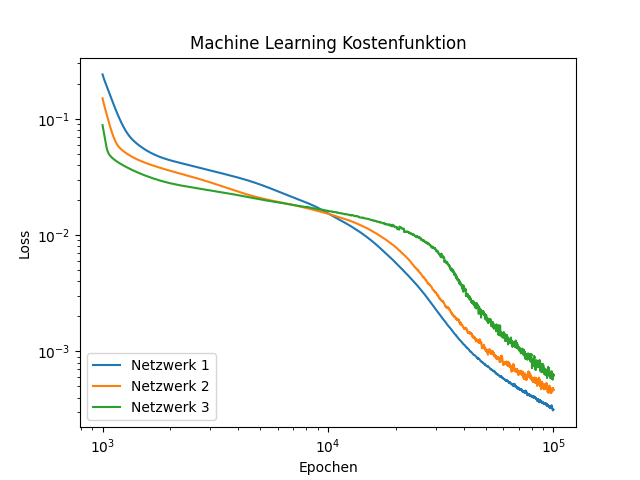
\includegraphics[scale=0.8]{harmonicoscillator_plots/harmonicoscillatorML_error__layers_var_avrloss}
       \caption{Kostenfunktion der verschiedenen neuronalen Netze.}
       \label{fig:harmonic-layers-variable-loss}
\end{figure}
\begin{figure}
       \centering
       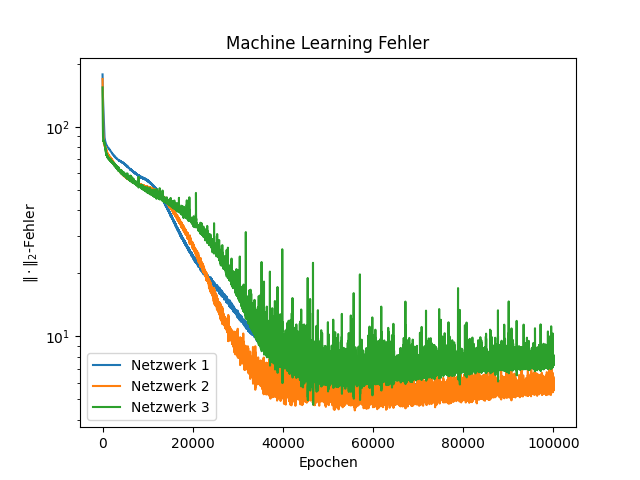
\includegraphics[scale=0.8]{harmonicoscillator_plots/harmonicoscillatorML_error__layers_var_error}
       \caption{Globaler Fehler der verschiedenen neuronalen Netze.}
       \label{fig:harmonic-layers-variable-error}
\end{figure}
\begin{figure}
       \centering
       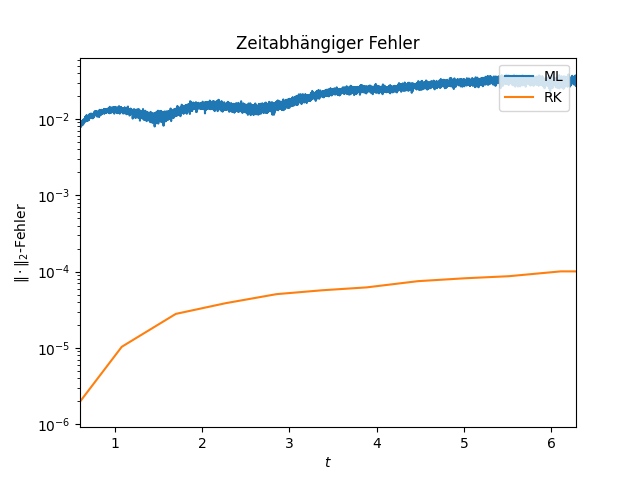
\includegraphics[scale=0.8]{harmonicoscillator_plots/harmonicoscillatorError_in_time_layers_var}
       \caption{Globaler Fehler von Netzwerken $1$ bis $3$ und dem Runge-Kutta-Verfahren in Abhängigkeit der Zeit.}
       \label{fig:harmonic-layers-variable-error-in-time}
\end{figure}
\begin{figure}
       \centering
       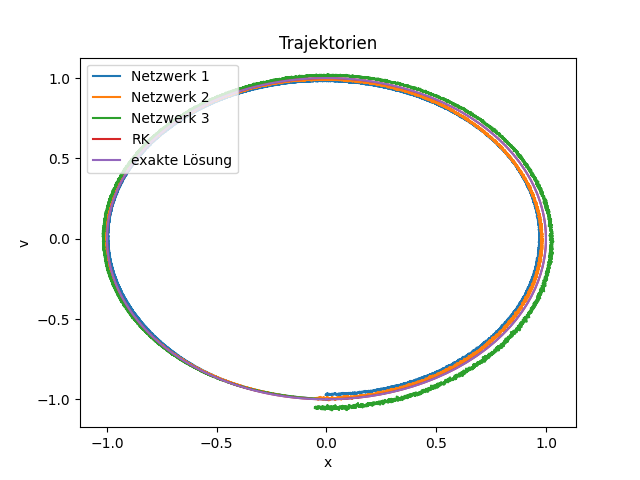
\includegraphics[scale=0.8]{harmonicoscillator_plots/harmonicoscillator_layers_vartrajectories}
       \caption{Trajektorien der von den verschiedenen neuronalen Netzen approximierte Lösung, der Runge-Kutta-Lösung
       und der exakten Lösung.}
       \label{fig:harmonic-layers-variable-trajectories}
\end{figure}
\begin{figure}
       \centering
       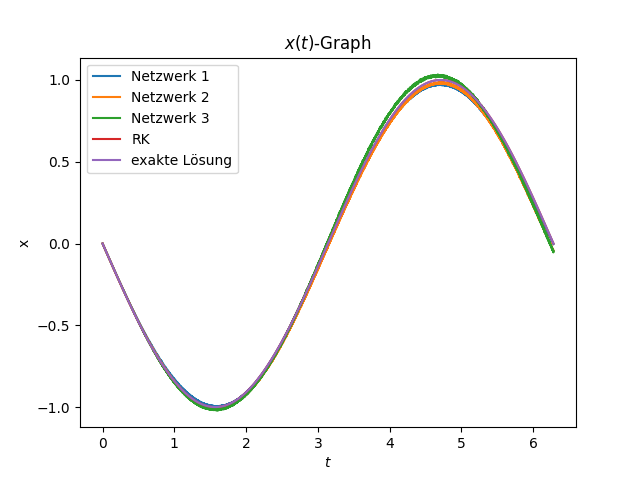
\includegraphics[scale=0.8]{harmonicoscillator_plots/harmonicoscillator_layers_vartrajectories_in_time_}
       \caption{$(t,x(t))$-Graph der von den verschiedenen neuronalen Netzen approximierte Lösung, der
       Runge-Kutta-Lösung und der exakten Lösung.}
       \label{fig:harmonic-layers-variable-trajectories-in-time}
\end{figure}
Zusammenfassend können wir also sagen, dass eine Erhöhung der Neuronen und Schichten abhängig von der Komplexität des
Anfangswertproblems ist. Außerdem muss die Trainingszeit erhöht werden, um eine vergleichbar gute Approximation
gegenüber dem Runge-Kutta-Verfahren zu erhalten.
\clearpage
